\begin{frame}
  \begin{block}{A. Arquitetura de Rede e Previsões de Trafego}
    \begin{itemize}
      \item A chegada de novas chamadas podem ser respondidas por ambas as redes.
      \item Parâmetros usados para decidir que rede deve ser escolhida:
      \begin{itemize}
        \item Consumo de energia
        \item Vazão
        \item Probabilidade de perda de pacote
      \end{itemize}
      \item Os serviços ofertados pela rede chegam no sistema de acordo com dois processos de Poisson
      \begin{itemize}
        \item Voz ($ \lambda v _{n} $)
        \item Dados ($ \lambda d _{n} $)
      \end{itemize}
      \item Os pacotes de chamadas de voz e dados seguem uma distribuição exponencial:$ 1 / \mu v _{n} $ and $ 1 / \mu d _{n} $,respectivamente
    \end{itemize}
  \end{block}
\end{frame}

\begin{frame}
  \begin{block}{B. Formulação do Problema}
    Objetivos do modelo markoviano proposto:
    \begin{itemize}
      \item Definir a qual rede o usuário móvel deve se conectar.
      \item Minimizar os custos dos parâmetros de:
      \item \alert{Energia}
      \item \alert{Perdas de transmissão}
      \item \alert{Baixa taxa de transferência}
    \end{itemize}  
  \end{block}  
\end{frame}

\begin{frame}
  \begin{block}{Possíveis eventos:}
    \begin{itemize}
      \scriptsize
      \item \alert{$\lambda v _{m}$} e \alert{$\lambda v _{f}$} - Taxa de chegada de voz na macrocell e femtocell
      \item \alert{$\lambda d _{m}$} e \alert{$\lambda d _{f}$} - Taxa de chegada de dados na macrocell e femtocell
      \item \alert{$\lambda v _{u}$} e \alert{$\lambda d _{u}$} - Taxa de chegadas de usuários para voz e dados
      \item \alert{$\mu v _{m}$}, \alert{$\mu v _{f}$} e \alert{$\mu v _{u}$} - Taxa de serviço para voz na macrocell, femtocell e alocação dos usuários
      \item \alert{$\mu d _{m}$}, \alert{$\mu d _{f}$} e \alert{$\mu d _{u}$} - Taxa de serviço para dados na macrocell, femtocell e alocação dos usuários
    \end{itemize}
  \end{block}
  
  \begin{block}{Parâmetros do sistema:}
    \begin{itemize}
      \scriptsize
      \item \alert{$v _{m}$} e \alert{$v _{f}$} - número de conexões de voz na macrocell e femtocell
      \item \alert{$d _{m}$} e \alert{$d _{f}$} - número de conexões de dados na macrocell e femtocell
      \item \alert{$c$} - estado de conexão do usuário: macrocell($c _{m}$), femtocell($c _{f}$) ou disconectado($disc$)
      \item \alert{$k$} - tipo de aplicação: $voz$, $dados$ ou $disc$
      \item \alert{$ev$} - último evento aguardando a decisão
    \end{itemize}
  \end{block}
\end{frame}

\begin{frame}
  \footnotesize Usando esses parâmetros, cada estado \alert{s $\epsilon$ S} é definido como uma 7-tupla:
  \begin{figure}
    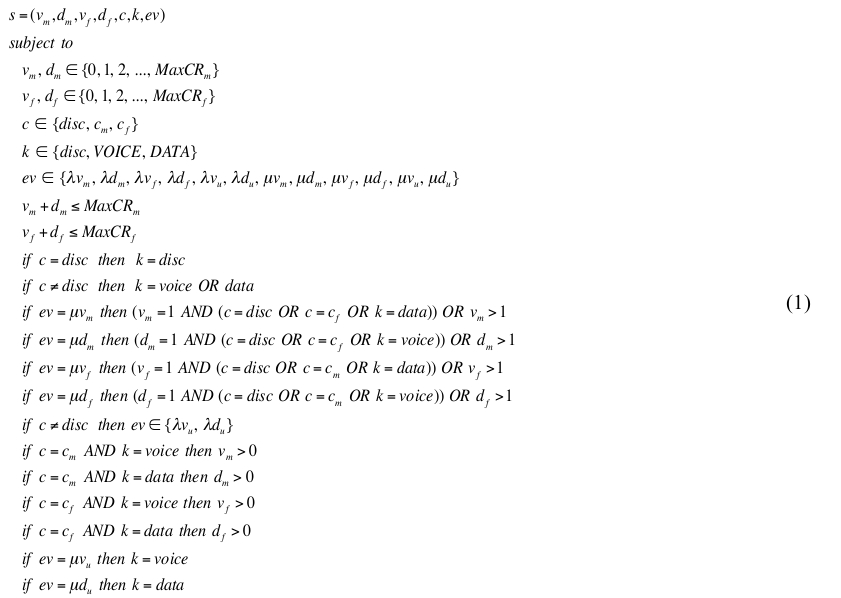
\includegraphics [scale=0.30]{./Figures/f1}
  \end{figure}
  \footnotesize Onde $MaxCR _{m}$ e $MaxCR _{f}$ são os números máximos de macrocell e femtocell, respectivamente  
\end{frame}

\begin{frame}
  \footnotesize O conjunto de possíveis ações \alert{$A(s)$} para cada estado \alert{s $\epsilon$ S} é definido como:
  \begin{figure}
    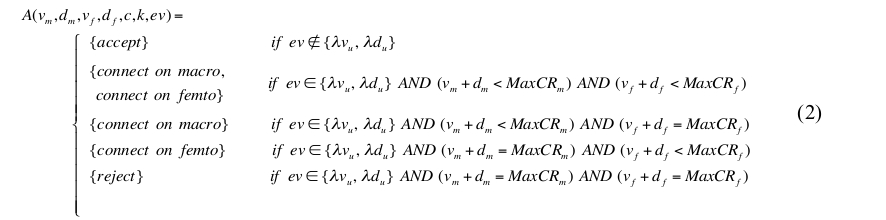
\includegraphics [scale=0.37]{./Figures/f2}
  \end{figure}  
\end{frame}

\begin{frame}
  \begin{itemize}
    \item Estados(\alert{$s _{t}$}) que podem ser alcançados a partir de \alert{$s _{f}$}
  \end{itemize}    
  \begin{figure}
    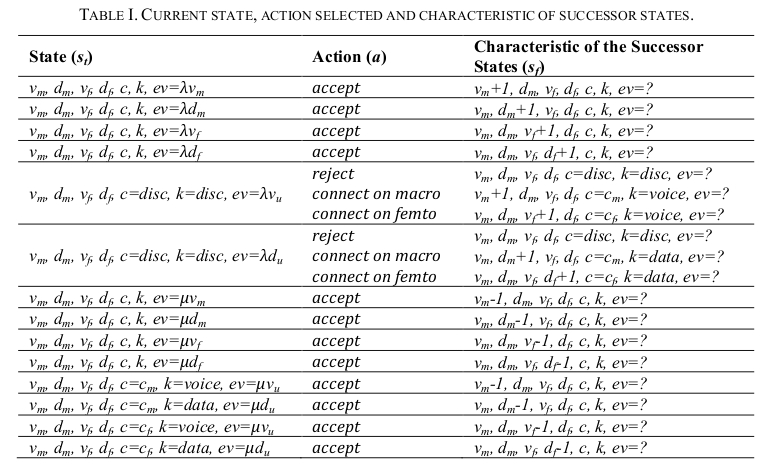
\includegraphics [scale=0.37]{./Figures/f3}
  \end{figure}  
\end{frame}

\begin{frame}
  \begin{itemize}
    \item Identificação dos possíveis estados que podem ser alcançados a partir de \alert{$s _{f}$}
  \end{itemize}    
  \begin{figure}
    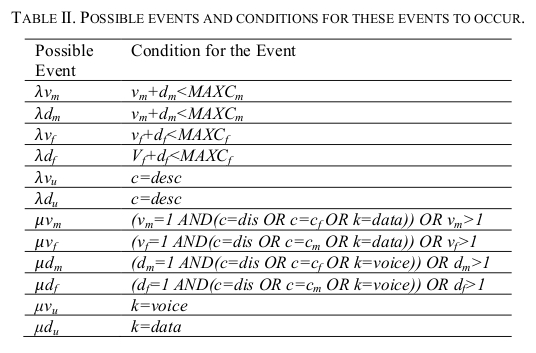
\includegraphics [scale=0.37]{./Figures/f4}
  \end{figure}  
\end{frame}

\begin{frame}{\small Como todos os eventos são representados por um processo de Poisson}
    \begin{itemize} 
      \item \footnotesize Cálculo da taxa de saída total \alert{$s _{f}$}, quando a ação \alert{$a$} é selecionada:
    \end{itemize} 
     
    \begin{figure} 
      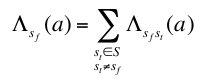
\includegraphics[scale=0.37]{./Figures/form1} 
      \scriptsize , onde $\Lambda _{sf st}$ é a taxa de transição do estado $s_{f}$ para o estado $s_{t}$.
    \end{figure}  
    
    \begin{itemize}
      \item \footnotesize Cálculo da probabilidade de transição:
    \end{itemize}
    
    \begin{figure} 
      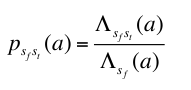
\includegraphics[scale=0.37]{./Figures/form2} 
    \end{figure}
    
    \begin{itemize}
      \item \footnotesize Cálculo do tempo esperado até a próxima decisão:
    \end{itemize}
    
    \begin{figure} 
      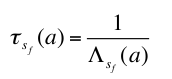
\includegraphics[scale=0.37]{./Figures/form3} 
    \end{figure}
\end{frame}

\begin{frame}
  \footnotesize Os custos utilizados pelo sistema quando este está no estado de \alert{$s_{f}$} e uma acção \alert{$a$} é escolhido, pode ser calculado por:
  \begin{figure}
    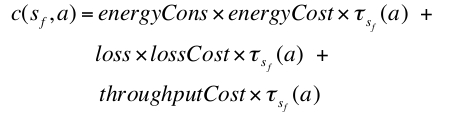
\includegraphics[scale=0.37]{./Figures/form4}
  \end{figure}
  \scriptsize Onde:
  \begin{itemize}
    \item \alert{$energyCons$} é o consumo de energia, podendo ser \alert{$energyCons_{m}$} ou \alert{$energyCons_{f}$}
    \item \alert{$energyCost$} é o custo energétio, podendo ser \alert{$energyCost_{m}$} ou \alert{$energyCost_{f}$}
    \item \alert{$loss$} é a probabilidade de perda de pacote, podendo ser \alert{$loss_{m}$} ou \alert {$loss_{f}$}
    \item \alert{$lossCost$} é o custo de energia, podendo ser \alert{$lossCost_{m}$} ou \alert{$lossCost_{m}$}
    \item \alert{$throuhputCost$} é o custo para transmitir com uma taxa de transferência reduzida
  \end{itemize}
\end{frame}
% \begin{frame}
%  \begin{block}{} 
%  \end{block}
% \end{frame}
%
% \begin{frame}
%  \begin{figure}[h]
%  	\begin{center}
%      \includegraphics [scale=0.3]{./Figures/Device-Estimates}
%     % \caption {Estimativa de dispositivos conectados à Internet.}
%  		%\label{fig:arq-imuno}
%  	\end{center}
%  \end{figure}
% \end{frame}
%
% \begin{frame}{Redes de Acesso}
% 	\begin{figure}[!htb]
% 		\centering
% 		\subfloat[DSL]{
% 			\includegraphics[height=3.5cm]{./Figures/DSLaccess}
% 			\label{figdroopy}}
% 		\quad %espaco separador
% 		\subfloat[Cable]{
% 			\includegraphics[height=3.5cm]{./Figures/CableAccess}
% 			\label{figsnoop}}
% 		%\caption{Subfiguras}
% 		%\label{fig01}
% 	\end{figure}
% \end{frame}
%
% \begin{frame}[fragile]
% \scriptsize
% \begin{verbatim}
% \end{verbatim}
% \end{frame}
